\documentclass[12pt]{fpgairpods}
\usepackage[letterpaper, margin=1in]{geometry}
\addbibresource{proposal.bib}
\graphicspath{{figs/}}

\setlist{noitemsep, topsep=0pt}

\begin{document}

{\Huge \textbf{FPGAirPods} Project Proposal}

\vspace{2mm}
{Gokul Kolady, Ben Kettle, Niko Ramirez | \today \ | 6.111}
\vspace{5mm}


\begin{multicols}{2}
\section{Overview}
Our 6.111 final project aims to implement active noise cancellation as seen in over- and in-ear headphones such as the Bose QC35 and the AirPods Pro (hence the name). In order to do this, we will first need to create a physical model of a single headphone (one ear cup) that we will use to test. Inside the ear cup, we will install a speaker (far from the ear) and a digital microphone (closer to the ear). We will also use a digital microphone external to the ear cup in order to capture ambient noise.

The FPGA itself will handle the computational side of the active noise cancellation. This will primarily involve an adaptive filter that will continually improve its coefficients in order to minimize the error function--ie, the noise that makes it through and is not cancelled out. We run the input from the external microphone through this filter, and play the filtered result out of the speaker with the aim of cancelling noise.

\section{Materials}


Several materials will be used in order to construct a prototype "headphone" to test on: 
\begin{itemize}
    \item 2x \href{https://www.adafruit.com/product/3421}{SPH0645LM4H microphone breakout boards} (\$7) from Adafruit will be used to collect noise from inside and outside the ear cup. These communicate via I2S, which will remove the need for ADCs between the microphone and the FPGA, and minimize potential for noise in the wires from the FPGA to the earpiece.
    \item 1x \href{https://www.adafruit.com/product/3968}{Speaker} (\$5) in order to play the anti-noise signal that we calculate into the user's ear. This is a 3W speaker, which should give adequate power.
    \item 1x \href{https://www.adafruit.com/product/3006}{I2S Amplifier} will be used to convert the digital output signal from the FPGA into an analog output signal to pass to the speaker.
    \item We will use a cup of some kind to mount all of these on.
    \item We'll create some passive noise insulation using some \href{https://www.amazon.com/Silverstone-21-Inch-Dampening-Acoustic-SF01/dp/B0040JHMH6?th=1}{foam}.
    \item We'll need some wire to connect the microphones and the speaker.
\end{itemize}

\end{multicols}


\begin{figure}
\def\svgwidth{\linewidth}
\input{./figs/system_diagram.pdf_tex}
\caption{The peripherals that will be included in our project}
\label{fig:peripherals}
\end{figure}

\begin{figure}
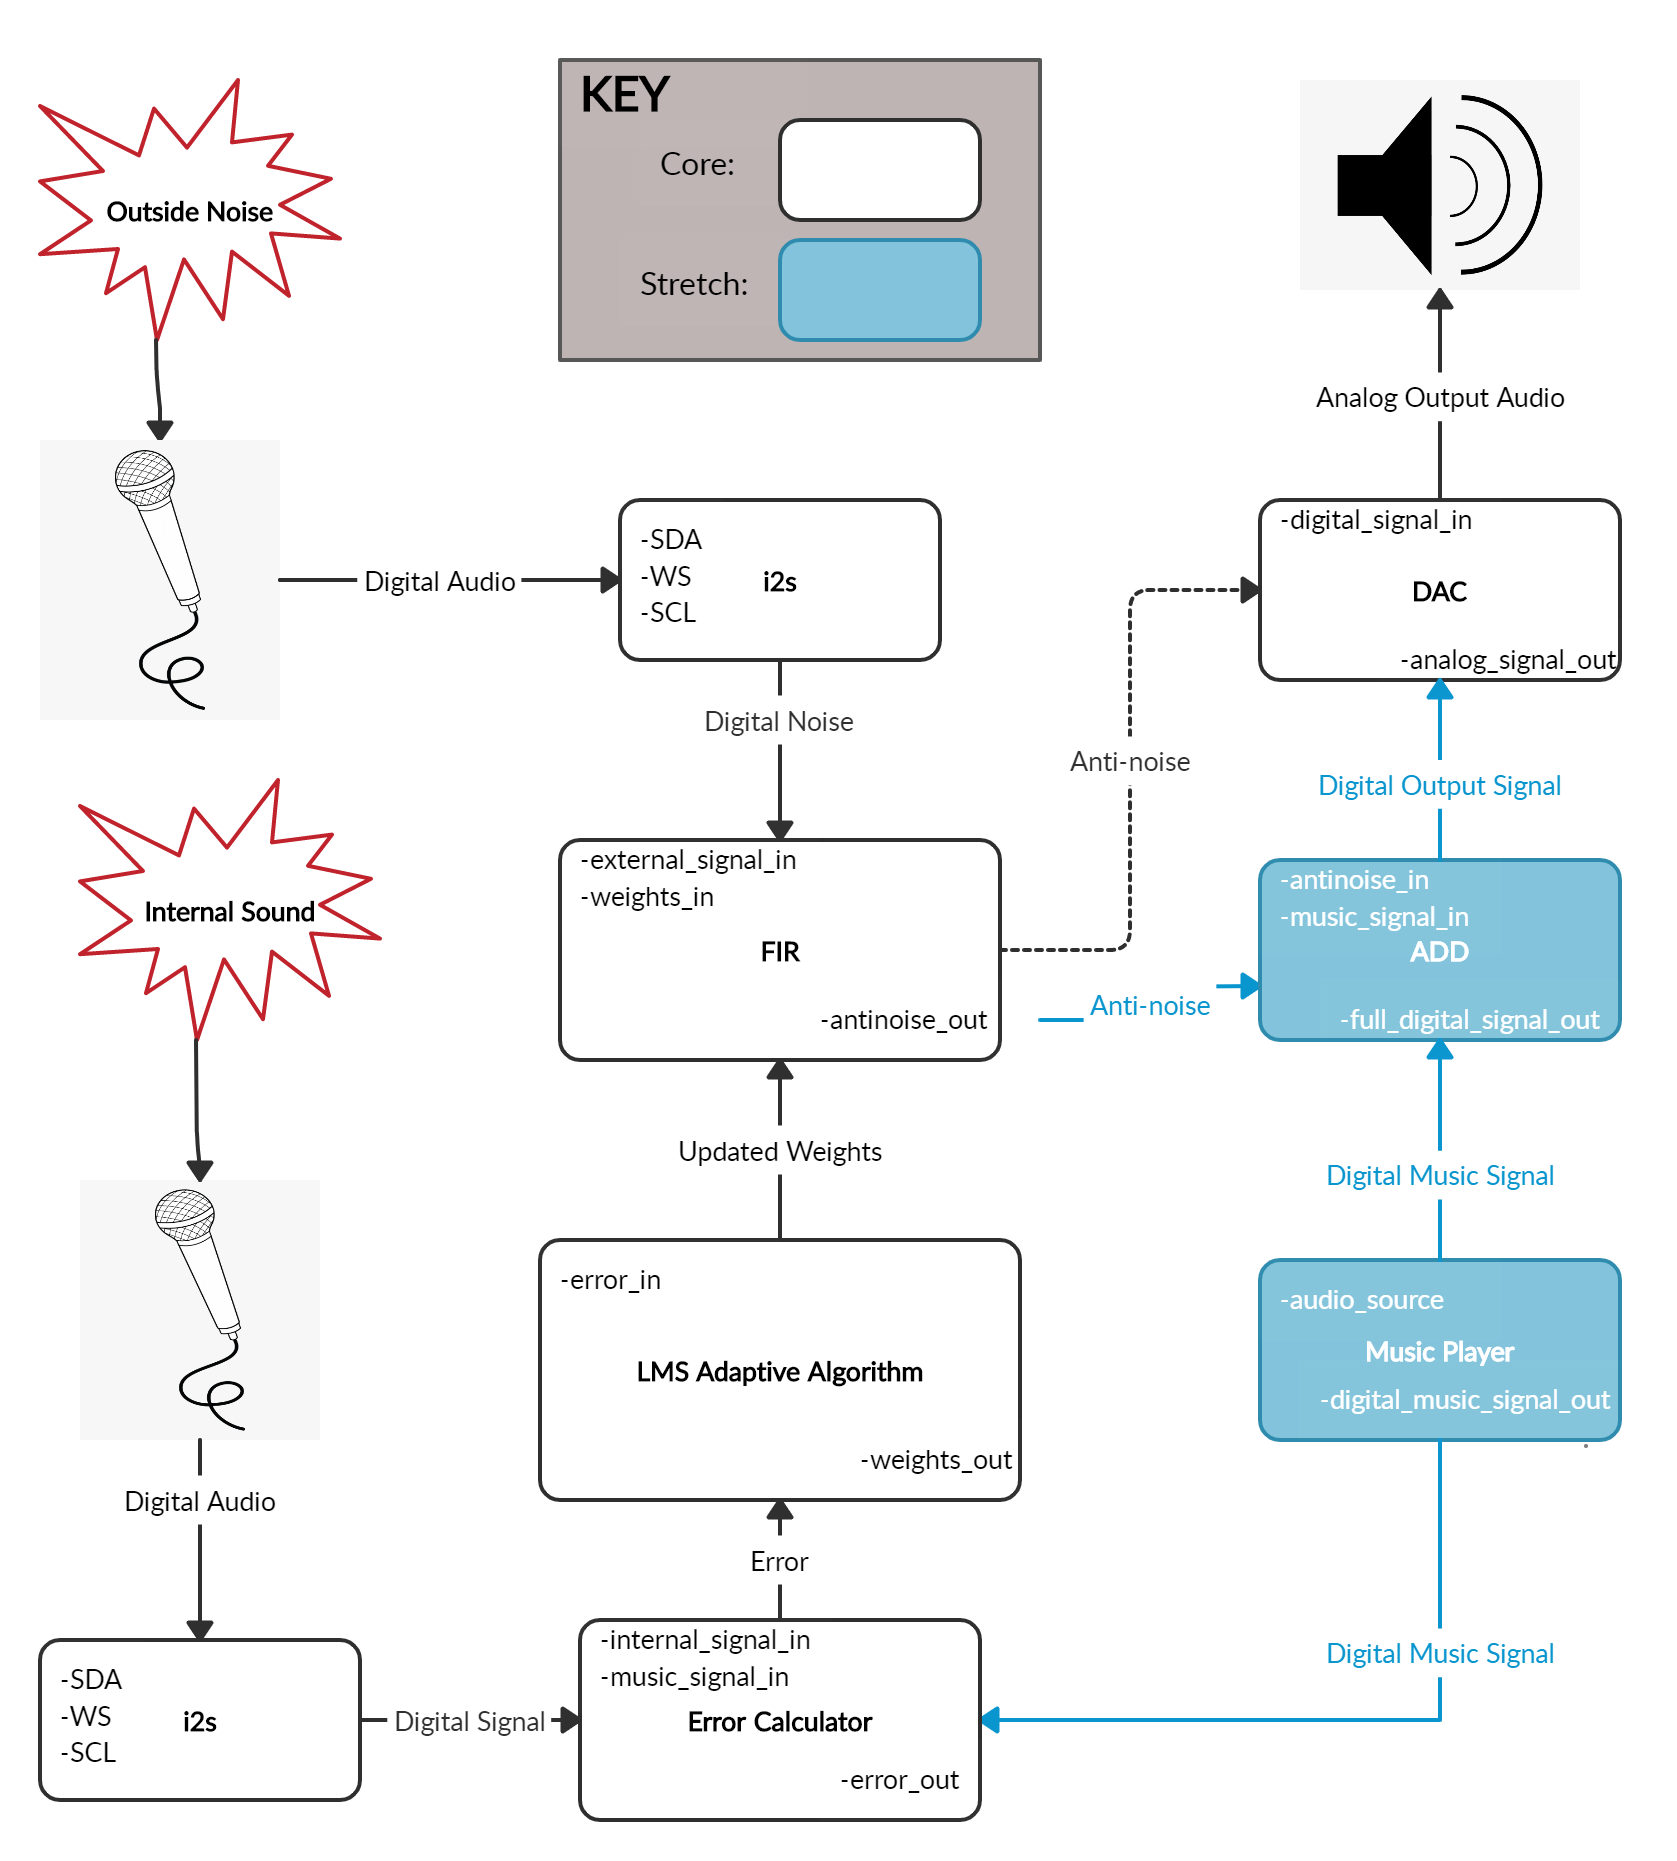
\includegraphics[width=\textwidth]{Proposal Block Diagram.png}
\caption{The high-level block diagram for our system.}
\label{fig:blockdiagram}
\end{figure}


\newpage
\section{Modules}
\begin{multicols}{2}
\subsection{I2S Receiver - \textit{IP}}
This module will parse the incoming data stream from each of the two microphones. We can either implement it using the Vivado I2S IP, or implement it ourselves. For our purposes, it may be more resource efficient to implement it ourselves.
\subsubsection{Inputs}
\begin{itemize}
    \item SDA - Microphone Data
    \item SCL - Audio Clock
\end{itemize}
\subsubsection{Outputs}
\subsubsection{Level of Performance}
\begin{itemize}
    \item 476 LUTs
    \item 1722 FFs
    \item 1 36k BRAM
\end{itemize}

\subsection{FIR Filter - \textit{Owners}}
The FIR Filter module convolves the external ambient noise with a set of filter coefficients in order to produce an anti-noise signal. This anti-noise signal is later used to cancel out the ambient noise that makes it into the the ear cup. These coefficients are set continuously by the LMS adaptive algorithm module.
\subsubsection{Inputs}
blah
\subsubsection{Outputs}
blah
\subsubsection{Complexity}
blah
\subsubsection{Level of Performance}
blah
\subsubsection{Testing}
blah
]
\subsection{LMS Adaptive Algorithm}
This module uses the LMS adaptive algorithm in order to update the coefficients of the FIR Filter for better noise cancellation. This algorithm takes advantage of the steepest descent optimization method, which analyzes the impact of the previous filter coefficients on the observed error and computes appropriate adjustments. This update is accomplished using the following equation, where $b_k(n)$ is the FIR coefficient for a given $k$ values and a given timestep $n$, $\Lambda$ is a predefined step size or learning rate that defines how quickly the filter weights change, and $f(n)$ is the value of the noise signal from the external microphone at a timestep $n$:

\[ b_k(n + 1) = b_k(n) + \Lambda e(n)f(n-k) \]
\[ k = 0, 1, 2,\ldots,  M-1 \]

\subsubsection{Inputs}
blah
\subsubsection{Outputs}
blah
\subsubsection{Complexity}
To implement this operation, we will need to store the last $M$ noise inputs from the external microphone along with the full last set of filter coefficients. This will require two BRAMs of size $w_S M$ and $w_C M$ respectively, where $w_S = 16$ is the bit depth of our samples from the external microphone, and $w_C$ is the bit depth of the coefficients.
\subsubsection{Level of Performance}
blah
\subsubsection{Testing}
Testing this module will be a bit more involved than some of the others due to its not well-defined behavior, but in order to test the behavior we will need to have a working FIR module. With this module in place, we can then test the ability of the LMS algorithm to recreate the coefficients of a given filter. In other words, we can have our "desired" signal be the result of passing some input through an arbitrary filter, use this desired signal to calculate the error $e(n)$, and pass this error into our LMS module. If the input of the LMS module is the same as the input to this mystery filter, 

\subsection{Error Calculator - \textit{Owners}}
The error calculator computes the difference between the output of the internal microphone (the sound within the ear cup) and the intended final audio. If we reach our stretch goal, the intended audio will be the music being inputted into the system. Otherwise, the goal will be silence. This difference or "error" will be fed into the LMS modules for error correction.
\subsubsection{Inputs}
blah
\subsubsection{Outputs}
blah
\subsubsection{Complexity}
blah
\subsubsection{Level of Performance}
blah
\subsubsection{Testing}
blah

\subsection{DAC - \textit{Owners}}
The DAC (Digital-to-Analog Converter) module will be used to transform the final digital output audio into an analog signal that can be played through the speaker.
\subsubsection{Inputs}
blah
\subsubsection{Outputs}
blah
\subsubsection{Complexity}
blah
\subsubsection{Level of Performance}
blah
\subsubsection{Testing}

\subsection{Music Player - \textit{Owners}}
This module outputs the source music/audio in digital form (the user should ideally hear a version of this audio with minimal corruption). With the possible extension of Bluetooth-based input audio, this module would be modified to receive its input from a Bluetooth receiver that would be interfaced with the FPGA.
\subsubsection{Inputs}
blah
\subsubsection{Outputs}
blah
\subsubsection{Complexity}
blah
\subsubsection{Level of Performance}
blah
\subsubsection{Testing}
blah

\subsection{Add - \textit{Owners}}
If we reach our stretch goal of the music player integration, we will need a module to merge the output of the FIR---the signal that will cancel the incoming noise---with the music to play. This module will take two signals as an input, and output their sum. It will be very simple.

\end{multicols}
Each module
\\-inputs and outputs
\\-complexity
\\-level of performance
\\(eg. number and type of arithmetic operations, size of internal memories, required throughput)
\\-how it will be tested

Teamwork Distribution
\\-team member works on which module 
\\-most modules should have a single designer
\\-testbenches should be different members

\printbibliography
\end{document}
